TODO: apraksti grafikiem un tabula līdz ko būs final version.

\section{Chatbot datu kopa}

\begin{table}[htbp]
  \centering
  \caption{Unikālo nodomu skaits "chatbot" treniņkopā un testa kopā.}
    \begin{tabular}{lrrr} \toprule
    Nodoms & Treniņkopā & Testa kopā & $\Sigma$ \\\midrule
    FindConnection & 57    & 71 & 128 \\
    DepartureTime & 43    & 35 & 78 \\
    $\Sigma$ & 100    & 106 & 206 \\\bottomrule
    \end{tabular}%
  \label{tab:chatbot-labels}%
\end{table}%


% Table generated by Excel2LaTeX from sheet 'chatbot_bert-base-multilingual-'
\begin{table}[htbp]
  \centering
  \caption{mBERT rezultāti}
    \begin{tabular}{lrrrrrr} \toprule
    languages & 1a & 1b & 2a & 2b & 3a & 3b \\\midrule
    % languages & 1\_translated & 1\_untranslated & 2\_translated & 2\_untranslated & 3\_translated & 3\_untranslated \\\midrule
    en    &   --  & 91.51 &  --   & 90.57 &  --   & 95.28 \\
    lv    & 90.57 & 88.68 & 94.34 & 93.40 & 92.45 & 85.85 \\
    ru    & 89.62 & 92.45 & 93.40 & 91.51 & 89.62 & 93.40 \\
    et    & 89.62 & 87.74 & 86.79 & 88.68 & 90.57 & 58.49 \\
    lt    & 95.28 & 94.34 & 94.34 & 94.34 & 91.51 & 79.25 \\\bottomrule
    \end{tabular}%
  \label{tab:chatbot-bert}%
\end{table}%

% Table generated by Excel2LaTeX from sheet 'chatbot_bert-base-multilingual-'
\begin{table}[htbp]
  \centering
  \caption{mBERT rezultāti}
    \begin{tabular}{lrrrrrr} \toprule
    languages & 1a & 1b & 2a & 2b & 3a & 3b \\\midrule
    % languages & 1\_translated & 1\_untranslated & 2\_translated & 2\_untranslated & 3\_translated & 3\_untranslated \\\midrule
    en    &  --   & \cellcolor[rgb]{ .988,  .988,  1}91.51 &    -- & \cellcolor[rgb]{ .984,  .969,  .98}90.57 &  --   & \cellcolor[rgb]{ .353,  .541,  .776}95.28 \\
    lv    & \cellcolor[rgb]{ .984,  .969,  .98}90.57 & \cellcolor[rgb]{ .984,  .937,  .949}88.68 & \cellcolor[rgb]{ .514,  .655,  .835}94.34 & \cellcolor[rgb]{ .671,  .765,  .89}93.40 & \cellcolor[rgb]{ .831,  .878,  .945}92.45 & \cellcolor[rgb]{ .984,  .886,  .898}85.85 \\
    ru    & \cellcolor[rgb]{ .984,  .953,  .965}89.62 & \cellcolor[rgb]{ .831,  .878,  .945}92.45 & \cellcolor[rgb]{ .671,  .765,  .89}93.40 & \cellcolor[rgb]{ .988,  .988,  1}91.51 & \cellcolor[rgb]{ .984,  .953,  .965}89.62 & \cellcolor[rgb]{ .671,  .765,  .89}93.40 \\
    et    & \cellcolor[rgb]{ .984,  .953,  .965}89.62 & \cellcolor[rgb]{ .984,  .922,  .933}87.74 & \cellcolor[rgb]{ .984,  .906,  .914}86.79 & \cellcolor[rgb]{ .984,  .937,  .949}88.68 & \cellcolor[rgb]{ .984,  .969,  .98}90.57 & \cellcolor[rgb]{ .973,  .412,  .42}58.49 \\
    lt    & \cellcolor[rgb]{ .353,  .541,  .776}95.28 & \cellcolor[rgb]{ .514,  .655,  .835}94.34 & \cellcolor[rgb]{ .514,  .655,  .835}94.34 & \cellcolor[rgb]{ .514,  .655,  .835}94.34 & \cellcolor[rgb]{ .988,  .988,  1}91.51 & \cellcolor[rgb]{ .98,  .773,  .784}79.25 \\\bottomrule
    \end{tabular}%
  \label{tab:chatbot-bert}%
\end{table}%


% Table generated by Excel2LaTeX from sheet 'chatbot_xlm-roberta-base_result'
\begin{table}[htbp]
  \centering
  \caption{Add caption}
    \begin{tabular}{lrrrrrr} \toprule
    languages & 1a & 1b & 2a & 2b & 3a & 3b \\\midrule
    % languages & 1\_translated & 1\_untranslated & 2\_translated & 2\_untranslated & 3\_translated & 3\_untranslated \\\midrule
    en    &   --  & 95.28 &   --  & 95.28 &  --   & 96.23 \\
    lv    & 91.51 & 88.68 & 93.40 & 93.40 & 94.34 & 85.85 \\
    ru    & 92.45 & 94.34 & 88.68 & 94.34 & 91.51 & 90.57 \\
    et    & 88.68 & 91.51 & 88.68 & 89.62 & 91.51 & 63.21 \\
    lt    & 92.45 & 91.51 & 91.51 & 93.40 & 90.57 & 77.36 \\\bottomrule
    \end{tabular}%
  \label{tab:chatbot-xlm}%
\end{table}%


% Table generated by Excel2LaTeX from sheet 'chatbot_xlm-roberta-base_result'
\begin{table}[htbp]
  \centering
  \caption{Add caption}
    \begin{tabular}{lrrrrrr} \toprule
    languages & 1a & 1b & 2a & 2b & 3a & 3b \\\midrule
    % languages & 1\_translated & 1\_untranslated & 2\_translated & 2\_untranslated & 3\_translated & 3\_untranslated \\\midrule
    en    &   --  & \cellcolor[rgb]{ .482,  .631,  .824}95.28 &  --   & \cellcolor[rgb]{ .482,  .631,  .824}95.28 &  --   & \cellcolor[rgb]{ .353,  .541,  .776}96.23 \\
    lv    & \cellcolor[rgb]{ .988,  .988,  1}91.51 & \cellcolor[rgb]{ .984,  .929,  .941}88.68 & \cellcolor[rgb]{ .737,  .812,  .914}93.40 & \cellcolor[rgb]{ .737,  .812,  .914}93.40 & \cellcolor[rgb]{ .608,  .722,  .867}94.34 & \cellcolor[rgb]{ .984,  .871,  .882}85.85 \\
    ru    & \cellcolor[rgb]{ .863,  .902,  .957}92.45 & \cellcolor[rgb]{ .608,  .722,  .867}94.34 & \cellcolor[rgb]{ .984,  .929,  .941}88.68 & \cellcolor[rgb]{ .608,  .722,  .867}94.34 & \cellcolor[rgb]{ .988,  .988,  1}91.51 & \cellcolor[rgb]{ .984,  .969,  .98}90.57 \\
    et    & \cellcolor[rgb]{ .984,  .929,  .941}88.68 & \cellcolor[rgb]{ .988,  .988,  1}91.51 & \cellcolor[rgb]{ .984,  .929,  .941}88.68 & \cellcolor[rgb]{ .984,  .949,  .961}89.62 & \cellcolor[rgb]{ .988,  .988,  1}91.51 & \cellcolor[rgb]{ .973,  .412,  .42}63.21 \\
    lt    & \cellcolor[rgb]{ .863,  .902,  .957}92.45 & \cellcolor[rgb]{ .988,  .988,  1}91.51 & \cellcolor[rgb]{ .988,  .988,  1}91.51 & \cellcolor[rgb]{ .737,  .812,  .914}93.40 & \cellcolor[rgb]{ .984,  .969,  .98}90.57 & \cellcolor[rgb]{ .98,  .698,  .71}77.36 \\\bottomrule
    \end{tabular}%
  \label{tab:chatbot-xlm}%
\end{table}%




\begin{figure}[h] 
   \centering
   \subcaptionbox{mBERT latviešu treniņdatu kopa}{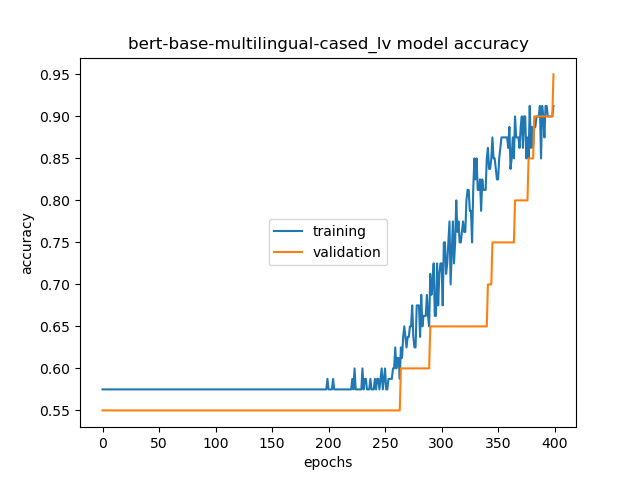
\includegraphics[width=0.49\linewidth,trim={0 0.1cm 0 0},clip]{graphs/bert-base-multilingual-cased_lv-accuracy.png}}
   \subcaptionbox{mBERT mašīntulkoto latviešu treniņdatu kopa}{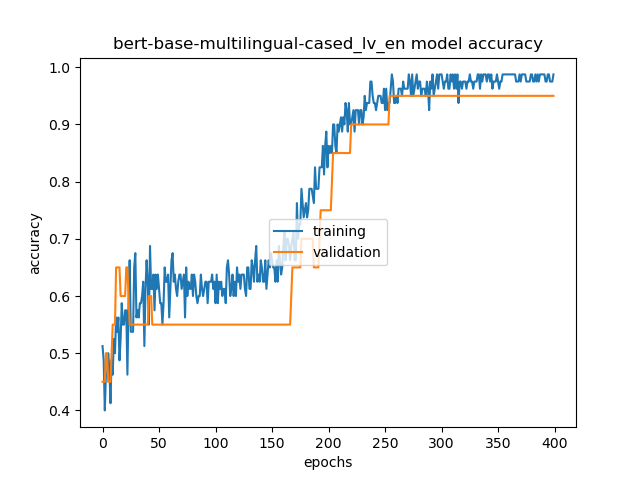
\includegraphics[width=0.49\linewidth,trim={0 0.1cm 0 0},clip]{graphs/bert-base-multilingual-cased_lv_en-accuracy.png}}
   \caption{caption} 
   \label{fig:chatbot-bert}
\end{figure}


\begin{figure}[h] 
   \centering
   \subcaptionbox{mBERT apvienotā treniņdatu kopa}{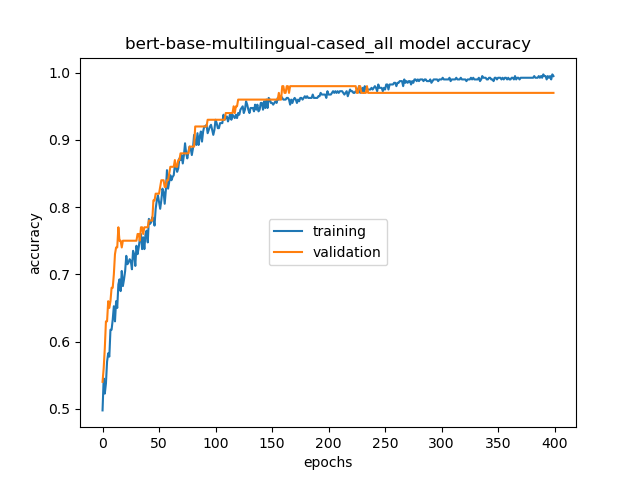
\includegraphics[width=0.49\linewidth,trim={0 0.1cm 0 0},clip]{graphs/bert-base-multilingual-cased_all-accuracy.png}}
   \subcaptionbox{mBERT apvienotā mašīntulkoto treniņdatu kopa}{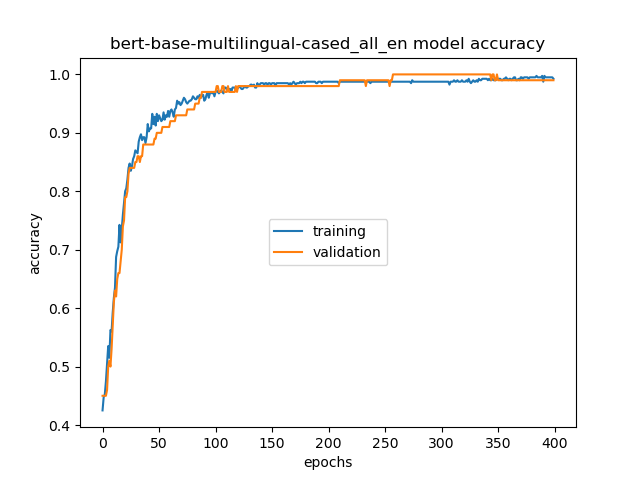
\includegraphics[width=0.49\linewidth,trim={0 0.1cm 0 0},clip]{graphs/bert-base-multilingual-cased_all_en-accuracy.png}}
   \caption{caption} 
   \label{fig:chatbot-bert-all}
\end{figure}


\begin{figure}[h] 
   \centering
   \subcaptionbox{mBERT angļu treniņdatu kopa}{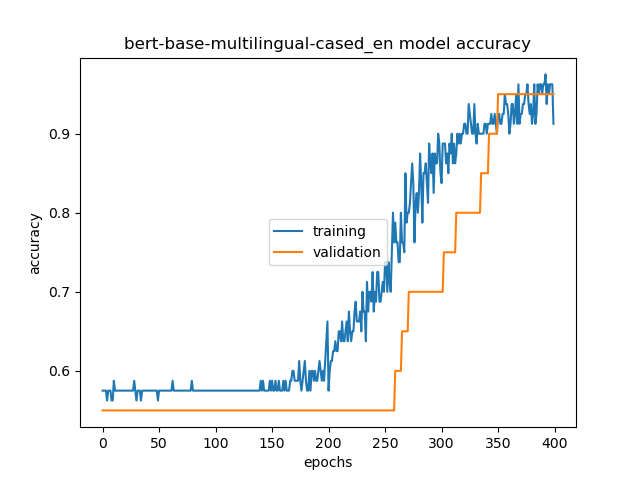
\includegraphics[width=0.49\linewidth,trim={0 0.1cm 0 0},clip]{graphs/bert-base-multilingual-cased_en-accuracy.png}}
   \subcaptionbox{XLM-RoBERTa angļu treniņdatu kopa}{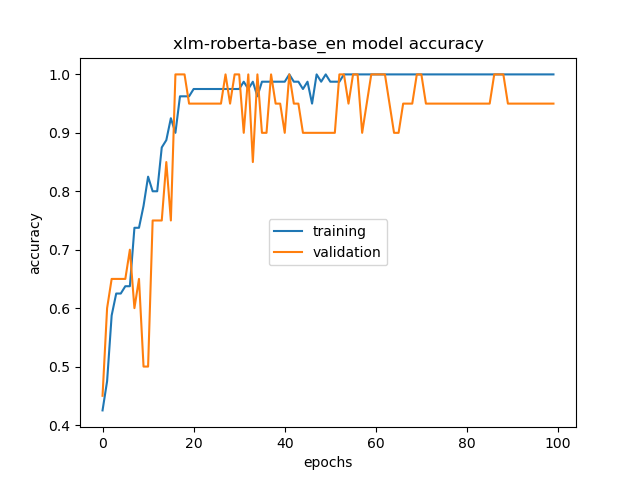
\includegraphics[width=0.49\linewidth,trim={0 0.1cm 0 0},clip]{graphs/xlm-roberta-base_en-accuracy.png}}
   \caption{caption} 
   \label{fig:chabot-bert-xlm-en}
\end{figure}


\begin{figure}[h] 
   \centering
   \subcaptionbox{XLM-RoBERTa latviešu treniņdatu kopa}{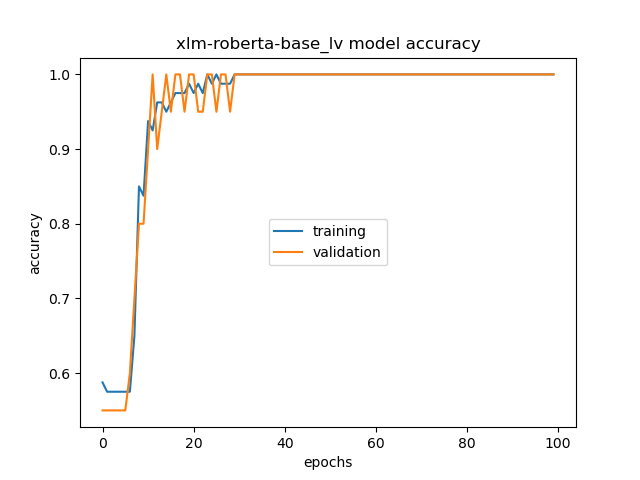
\includegraphics[width=0.49\linewidth,trim={0 0.1cm 0 0},clip]{graphs/xlm-roberta-base_lv-accuracy.png}}
   \subcaptionbox{XLM-RoBERTa mašīntulkoto latviešu treniņdatu kopa}{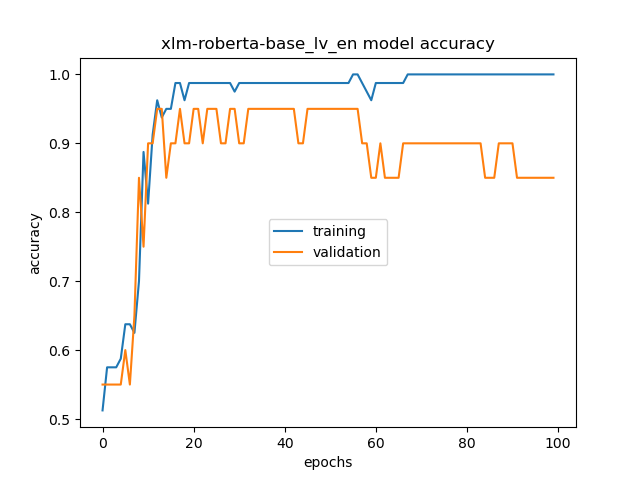
\includegraphics[width=0.49\linewidth,trim={0 0.1cm 0 0},clip]{graphs/xlm-roberta-base_lv_en-accuracy.png}}
   \caption{caption} 
   \label{fig:chatbot-xlm}
\end{figure}


\begin{figure}[h] 
   \centering
   \subcaptionbox{XLM-RoBERTa apvienotā treniņdatu kopa}{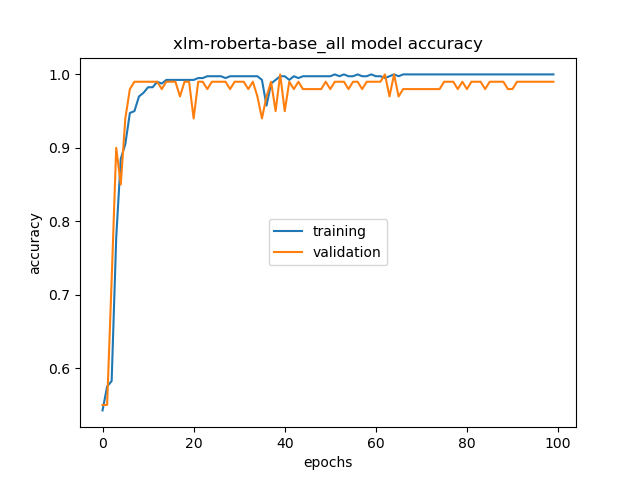
\includegraphics[width=0.49\linewidth,trim={0 0.1cm 0 0},clip]{graphs/xlm-roberta-base_all-accuracy.png}}
   \subcaptionbox{XLM-RoBERTa apvienotā mašīntulkoto treniņdatu kopa}{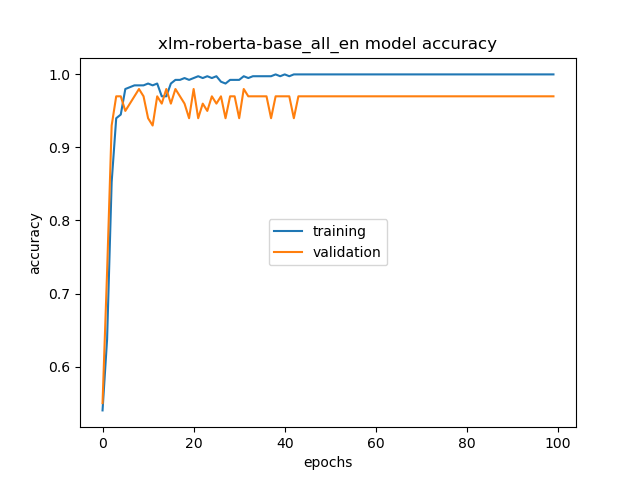
\includegraphics[width=0.49\linewidth,trim={0 0.1cm 0 0},clip]{graphs/xlm-roberta-base_all_en-accuracy.png}}
   \caption{caption} 
   \label{fig:chatbot-xlm-all}
\end{figure}


\section{Askubuntu datu kopa}

\begin{table}[htbp]
  \centering
  \caption{Unikālo nodomu skaits "askubuntu" treniņkopā un testa kopā.}
    \begin{tabular}{lrrr} \toprule
    Nodoms & Treniņkopā & Testa kopā & $\Sigma$ \\\midrule
    Software Recommendation & 17    & 40 & 57 \\
    Make Update & 10    & 37 & 47 \\
    Shutdown Computer & 13    & 14 & 27 \\
    Setup Printer & 10    & 13 & 23\\
    None  & 3     & 5 & 8\\
   $\Sigma$ & 53    & 109 & 162 \\\bottomrule
    \end{tabular}%
  \label{tab:askubuntu-labels}%
\end{table}%


% Table generated by Excel2LaTeX from sheet 'askubuntu_bert-base-multilingua'
\begin{table}[htbp]
  \centering
  \caption{Askubuntu rezultāti ar mBERT modeli}
    \begin{tabular}{lrrrrrr} \toprule
    languages & 1a & 1b & 2a & 2b & 3a & 3b \\\midrule
    % languages & 1\_translated & 1\_untranslated & 2\_translated & 2\_untranslated & 3\_translated & 3\_untranslated \\\midrule
    en    &  --   & \cellcolor[rgb]{ .984,  .965,  .976}78.90 &   --  & \cellcolor[rgb]{ .737,  .812,  .914}81.65 &  --   & \cellcolor[rgb]{ .608,  .722,  .867}82.57 \\
    lv    & \cellcolor[rgb]{ .984,  .965,  .976}78.90 & \cellcolor[rgb]{ .737,  .812,  .914}81.65 & \cellcolor[rgb]{ .988,  .988,  1}79.82 & \cellcolor[rgb]{ .353,  .541,  .776}84.40 & \cellcolor[rgb]{ .863,  .902,  .957}80.73 & \cellcolor[rgb]{ .973,  .412,  .42}54.13 \\
    ru    & \cellcolor[rgb]{ .482,  .631,  .824}83.49 & \cellcolor[rgb]{ .737,  .812,  .914}81.65 & \cellcolor[rgb]{ .984,  .882,  .894}75.23 & \cellcolor[rgb]{ .737,  .812,  .914}81.65 & \cellcolor[rgb]{ .988,  .988,  1}79.82 & \cellcolor[rgb]{ .976,  .655,  .667}65.14 \\
    et    & \cellcolor[rgb]{ .984,  .965,  .976}78.90 & \cellcolor[rgb]{ .482,  .631,  .824}83.49 & \cellcolor[rgb]{ .737,  .812,  .914}81.65 & \cellcolor[rgb]{ .984,  .925,  .937}77.06 & \cellcolor[rgb]{ .984,  .965,  .976}78.90 & \cellcolor[rgb]{ .973,  .494,  .502}57.80 \\
    lt    & \cellcolor[rgb]{ .608,  .722,  .867}82.57 & \cellcolor[rgb]{ .984,  .945,  .957}77.98 & \cellcolor[rgb]{ .984,  .965,  .976}78.90 & \cellcolor[rgb]{ .98,  .824,  .831}72.48 & \cellcolor[rgb]{ .863,  .902,  .957}80.73 & \cellcolor[rgb]{ .973,  .533,  .541}59.63 \\\bottomrule
    \end{tabular}%
  \label{tab:askubuntu-bert}%
\end{table}%

% uncolored just in case
% Table generated by Excel2LaTeX from sheet 'askubuntu_bert-base-multilingua'
\begin{table}[htbp]
  \centering
  \caption{Askubuntu rezultāti ar mBERT modeli}
    \begin{tabular}{lrrrrrr} \toprule
    languages & 1a & 1b & 2a & 2b & 3a & 3b \\\midrule
    % languages & 1\_translated & 1\_untranslated & 2\_translated & 2\_untranslated & 3\_translated & 3\_untranslated \\\midrule
    en    &   --  & 78.90 &   --  & 81.65 &  --   & 82.57 \\
    lv    & 78.90 & 81.65 & 79.82 & 84.40 & 80.73 & 54.13 \\
    ru    & 83.49 & 81.65 & 75.23 & 81.65 & 79.82 & 65.14 \\
    et    & 78.90 & 83.49 & 81.65 & 77.06 & 78.90 & 57.80 \\
    lt    & 82.57 & 77.98 & 78.90 & 72.48 & 80.73 & 59.63 \\\bottomrule
    \end{tabular}%
  \label{tab:askubuntu-bert}%
\end{table}%


% Table generated by Excel2LaTeX from sheet 'askubuntu_xlm-roberta-base_resu'
\begin{table}[htbp]
  \centering
  \caption{Askubuntu rezultāti ar XLM-RoBERTa modeli}
    \begin{tabular}{lrrrrrr}\toprule
    languages & 1a & 1b & 2a & 2b & 3a & 3b \\\midrule
    % languages & 1\_translated & 1\_untranslated & 2\_translated & 2\_untranslated & 3\_translated & 3\_untranslated \\\midrule
    en    &   --  & \cellcolor[rgb]{ .498,  .643,  .827}77.06 &  --   & \cellcolor[rgb]{ .353,  .541,  .776}78.90 &   --  & \cellcolor[rgb]{ .988,  .988,  1}70.64 \\
    lv    & \cellcolor[rgb]{ .984,  .922,  .933}67.89 & \cellcolor[rgb]{ .98,  .816,  .827}63.30 & \cellcolor[rgb]{ .353,  .541,  .776}78.90 & \cellcolor[rgb]{ .353,  .541,  .776}78.90 & \cellcolor[rgb]{ .639,  .741,  .878}75.23 & \cellcolor[rgb]{ .973,  .451,  .459}47.71 \\
    ru    & \cellcolor[rgb]{ .984,  .922,  .933}67.89 & \cellcolor[rgb]{ .78,  .843,  .929}73.39 & \cellcolor[rgb]{ .639,  .741,  .878}75.23 & \cellcolor[rgb]{ .639,  .741,  .878}75.23 & \cellcolor[rgb]{ .98,  .835,  .847}64.22 & \cellcolor[rgb]{ .976,  .561,  .569}52.29 \\
    et    & \cellcolor[rgb]{ .984,  .878,  .89}66.06 & \cellcolor[rgb]{ .984,  .965,  .976}69.72 & \cellcolor[rgb]{ .78,  .843,  .929}73.39 & \cellcolor[rgb]{ .353,  .541,  .776}78.90 & \cellcolor[rgb]{ .984,  .859,  .871}65.14 & \cellcolor[rgb]{ .973,  .494,  .502}49.54 \\
    lt    & \cellcolor[rgb]{ .984,  .965,  .976}69.72 & \cellcolor[rgb]{ .98,  .835,  .847}64.22 & \cellcolor[rgb]{ .427,  .592,  .804}77.98 & \cellcolor[rgb]{ .71,  .792,  .902}74.31 & \cellcolor[rgb]{ .988,  .988,  1}70.64 & \cellcolor[rgb]{ .973,  .412,  .42}45.87 \\
    \end{tabular}%
  \label{tab:askubuntu-xlm}%
\end{table}%




% Table generated by Excel2LaTeX from sheet 'askubuntu_xlm-roberta-base_resu'
\begin{table}[htbp]
  \centering
  \caption{Askubuntu rezultāti ar XLM-RoBERTa modeli}
    \begin{tabular}{lrrrrrr}\toprule
    languages & 1a & 1b & 2a & 2b & 3a & 3b \\\midrule
    % languages & 1\_translated & 1\_untranslated & 2\_translated & 2\_untranslated & 3\_translated & 3\_untranslated \\\midrule
    en    &   --  & 77.06 &  --   & 78.90 &  --   & 70.64 \\
    lv    & 67.89 & 63.30 & 78.90 & 78.90 & 75.23 & 47.71 \\
    ru    & 67.89 & 73.39 & 75.23 & 75.23 & 64.22 & 52.29 \\
    et    & 66.06 & 69.72 & 73.39 & 78.90 & 65.14 & 49.54 \\
    lt    & 69.72 & 64.22 & 77.98 & 74.31 & 70.64 & 45.87 \\\bottomrule
    \end{tabular}%
  \label{tab:askubuntu-xlm}%
\end{table}%



\begin{figure}[h] 
   \centering
   \subcaptionbox{mBERT latviešu treniņdatu kopa}{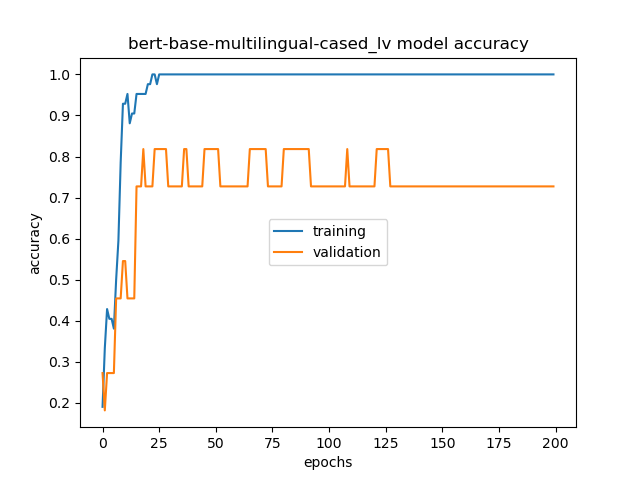
\includegraphics[width=0.49\linewidth,trim={0 0.1cm 0 0},clip]{results-5/graphs/askubuntu_bert-base-multilingual-cased_lv-accuracy.png}}
   \subcaptionbox{mBERT mašīntulkoto latviešu treniņdatu kopa}{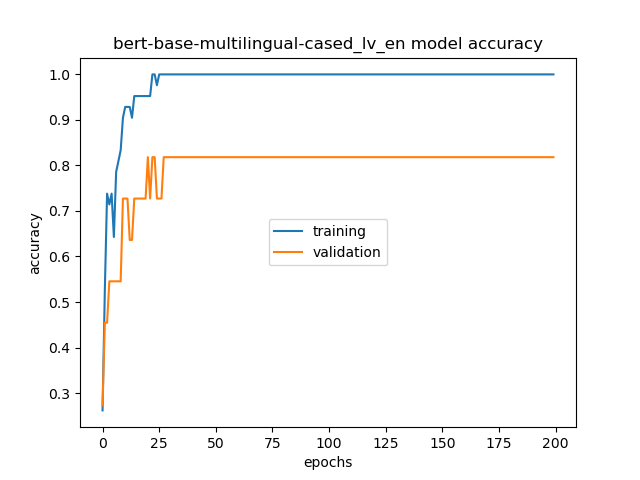
\includegraphics[width=0.49\linewidth,trim={0 0.1cm 0 0},clip]{results-5/graphs/askubuntu_bert-base-multilingual-cased_lv_en-accuracy.png}}
   \caption{caption} 
   \label{fig:askubuntu-bert}
\end{figure}


\begin{figure}[h] 
   \centering
   \subcaptionbox{mBERT apvienotā treniņdatu kopa}{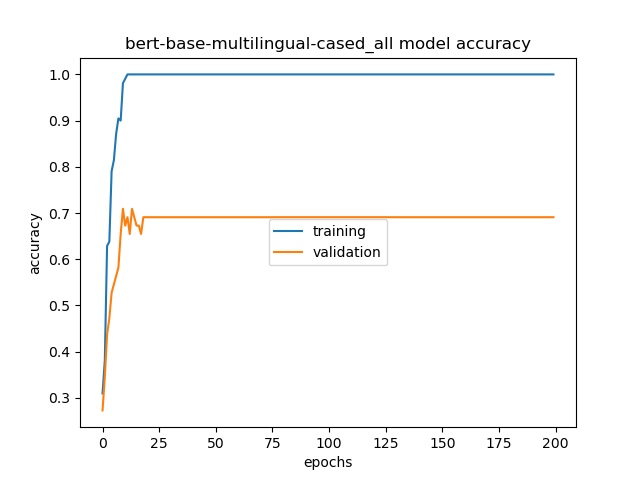
\includegraphics[width=0.49\linewidth,trim={0 0.1cm 0 0},clip]{results-5/graphs/askubuntu_bert-base-multilingual-cased_all-accuracy.png}}
   \subcaptionbox{mBERT apvienotā mašīntulkoto treniņdatu kopa}{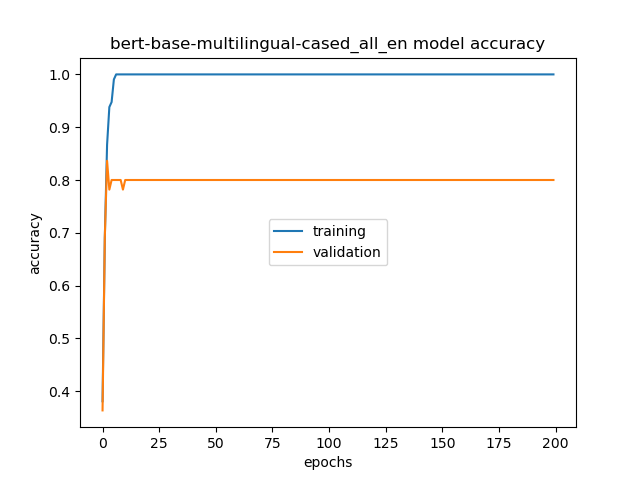
\includegraphics[width=0.49\linewidth,trim={0 0.1cm 0 0},clip]{results-5/graphs/askubuntu_bert-base-multilingual-cased_all_en-accuracy.png}}
   \caption{caption} 
   \label{fig:askubuntu-bert-all}
\end{figure}


\begin{figure}[h] 
   \centering
   \subcaptionbox{mBERT angļu treniņdatu kopa}{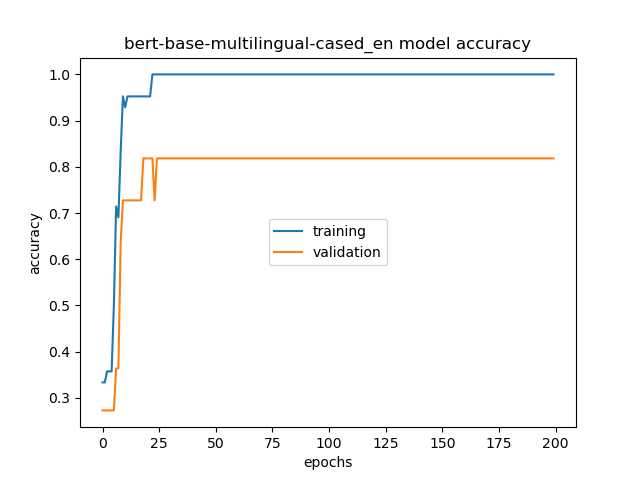
\includegraphics[width=0.49\linewidth,trim={0 0.1cm 0 0},clip]{results-5/graphs/askubuntu_bert-base-multilingual-cased_en-accuracy.png}}
   \subcaptionbox{XLM-RoBERTa angļu treniņdatu kopa}{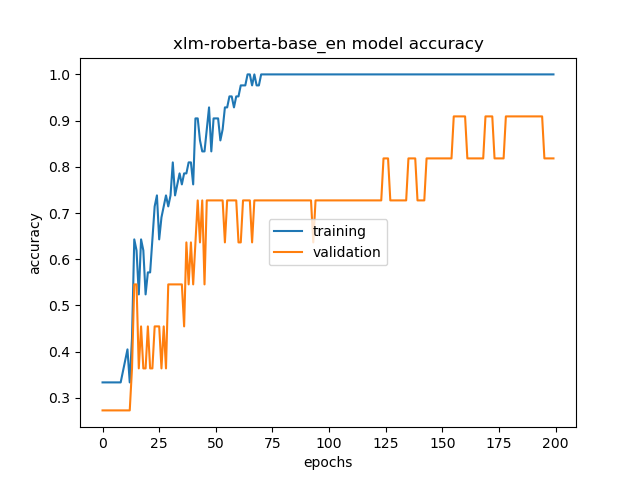
\includegraphics[width=0.49\linewidth,trim={0 0.1cm 0 0},clip]{results-5/graphs/askubuntu_xlm-roberta-base_en-accuracy.png}}
   \caption{caption} 
   \label{fig:askubuntu-bert-xlm-en}
\end{figure}


\begin{figure}[h] 
   \centering
   \subcaptionbox{XLM-RoBERTa latviešu treniņdatu kopa}{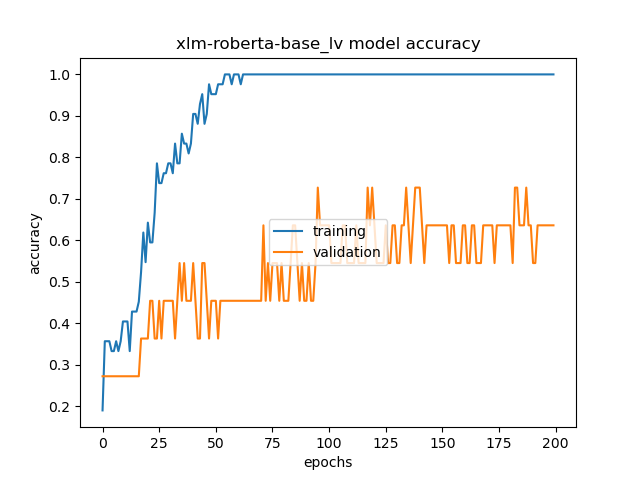
\includegraphics[width=0.49\linewidth,trim={0 0.1cm 0 0},clip]{results-5/graphs/askubuntu_xlm-roberta-base_lv-accuracy.png}}
   \subcaptionbox{XLM-RoBERTa mašīntulkoto latviešu treniņdatu kopa}{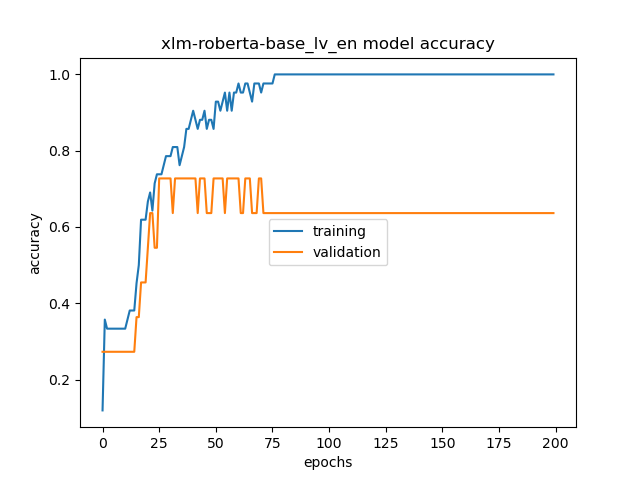
\includegraphics[width=0.49\linewidth,trim={0 0.1cm 0 0},clip]{results-5/graphs/askubuntu_xlm-roberta-base_lv_en-accuracy.png}}
   \caption{caption} 
   \label{fig:askubuntu-xlm}
\end{figure}


\begin{figure}[h] 
   \centering
   \subcaptionbox{XLM-RoBERTa apvienotā treniņdatu kopa}{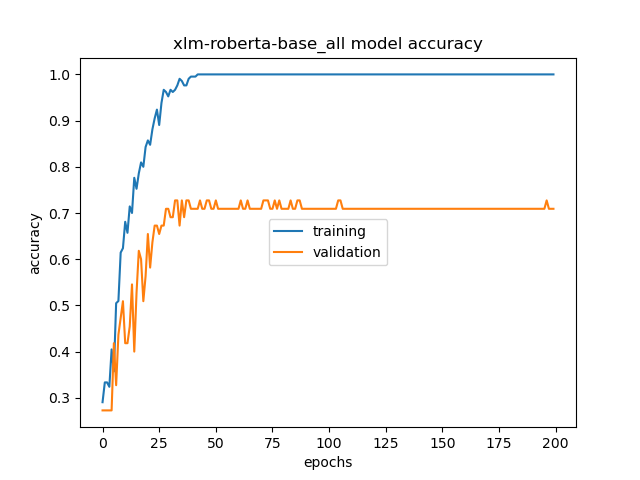
\includegraphics[width=0.49\linewidth,trim={0 0.1cm 0 0},clip]{results-5/graphs/askubuntu_xlm-roberta-base_all-accuracy.png}}
   \subcaptionbox{XLM-RoBERTa apvienotā mašīntulkoto treniņdatu kopa}{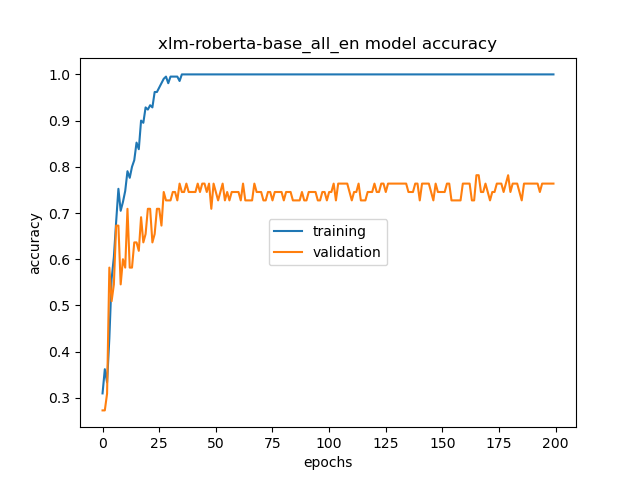
\includegraphics[width=0.49\linewidth,trim={0 0.1cm 0 0},clip]{results-5/graphs/askubuntu_xlm-roberta-base_all_en-accuracy.png}}
   \caption{caption} 
   \label{fig:askubuntu-xlm-all}
\end{figure}



\section{Webapps datu kopa}


Webapps datu kopā ir nodoms ar tikai vienu piemēru, kas izraisa "ValueError: The least populated class in y has only 1 member, which is too few. The minimum number of groups for any class cannot be less than 2." Tāpēc nodomi ar mazāk nekā trīs piemēriem tika apvienoti vienā nodomā "Other". Tas atbilst reālam pielietojumam industrijā, kur nodomi nav vienlīdzīgi pārstāvēti  -- piemēram, starp 115 dažādiem nodomiem divi visbiežākie nodomi kopā pārstāv 33\% datu kopas \cite{paikens2020} -- un ir svarīgi spēt atsijāt nodomus, kurus jāapstrādā klientu apkalpošanas speciālistam -- cilvēkam.



\begin{table}[htbp]
  \centering
  \caption{Unikālo nodomu skaits ``webapps" treniņkopā un testa kopā. Ar treknrakstu iezīmētas nodomi, kuri ir pietiekami pārstāvētas, pārējie nodomi tika apvienoti vienā jaunā nodomā: "Other"}
    \begin{tabular}{lrrr} \toprule
    Nodoms & Treniņkopā & Testa kopā & $\Sigma$ \\\midrule
    \textbf{Find Alternative} & \textbf{7} & \textbf{16} & 23\\
    \textbf{Delete Account} & \textbf{7} & \textbf{10} & 17\\
    \textbf{Filter Spam} & \textbf{6} & \textbf{14} & 20 \\
    \textbf{Sync Accounts} & \textbf{3} & \textbf{6} & 9 \\
    Change Password & 2     & 6 & 8\\
    None  & 2     & 4 & 6\\
    Export Data & 2     & 3 & 5 \\
    Download Video & 1     & 0 & 1\\
    $\Sigma$ & 30    & 59 & 89 \\\bottomrule
    \end{tabular}%
  \label{tab:webapps-labels}%
\end{table}%


% Table generated by Excel2LaTeX from sheet 'webapps_bert-base-multilingual-'
\begin{table}[htbp]
  \centering
  \caption{Webapps rezultāti ar mBERT modeli}
    \begin{tabular}{lrrrrrr}\toprule
    languages & 1a & 1b & 2a & 2b & 3a & 3b \\\midrule
    % languages & 1\_translated & 1\_untranslated & 2\_translated & 2\_untranslated & 3\_translated & 3\_untranslated \\\midrule
    en    &   --  & 64.41 &   --  & 67.80 &  --   & 61.02 \\
    lv    & 67.80 & 57.63 & 64.41 & 66.10 & 69.49 & 30.51 \\
    ru    & 67.80 & 69.49 & 72.88 & 74.58 & 64.41 & 44.07 \\
    et    & 55.93 & 61.02 & 67.80 & 71.19 & 69.49 & 42.37 \\
    lt    & 62.71 & 49.15 & 67.80 & 66.10 & 66.10 & 28.81 \\\bottomrule
    \end{tabular}%
  \label{tab:webapps-bert}%
\end{table}%


% Table generated by Excel2LaTeX from sheet 'webapps_bert-base-multilingual-'
\begin{table}[htbp]
  \centering
  \caption{Webapps rezultāti ar mBERT modeli}
    \begin{tabular}{lrrrrrr}\toprule
    languages & 1a & 1b & 2a & 2b & 3a & 3b \\\midrule
    % languages & 1\_translated & 1\_untranslated & 2\_translated & 2\_untranslated & 3\_translated & 3\_untranslated \\\midrule
    en    &   --  & \cellcolor[rgb]{ .984,  .961,  .973}64.41 &  --   & \cellcolor[rgb]{ .863,  .902,  .957}67.80 &   --  & \cellcolor[rgb]{ .984,  .906,  .918}61.02 \\
    lv    & \cellcolor[rgb]{ .863,  .902,  .957}67.80 & \cellcolor[rgb]{ .984,  .855,  .867}57.63 & \cellcolor[rgb]{ .984,  .961,  .973}64.41 & \cellcolor[rgb]{ .988,  .988,  1}66.10 & \cellcolor[rgb]{ .737,  .812,  .914}69.49 & \cellcolor[rgb]{ .973,  .435,  .443}30.51 \\
    ru    & \cellcolor[rgb]{ .863,  .902,  .957}67.80 & \cellcolor[rgb]{ .737,  .812,  .914}69.49 & \cellcolor[rgb]{ .482,  .631,  .824}72.88 & \cellcolor[rgb]{ .353,  .541,  .776}74.58 & \cellcolor[rgb]{ .984,  .961,  .973}64.41 & \cellcolor[rgb]{ .976,  .647,  .655}44.07 \\
    et    & \cellcolor[rgb]{ .98,  .827,  .839}55.93 & \cellcolor[rgb]{ .984,  .906,  .918}61.02 & \cellcolor[rgb]{ .863,  .902,  .957}67.80 & \cellcolor[rgb]{ .608,  .722,  .867}71.19 & \cellcolor[rgb]{ .737,  .812,  .914}69.49 & \cellcolor[rgb]{ .976,  .62,  .627}42.37 \\
    lt    & \cellcolor[rgb]{ .984,  .933,  .945}62.71 & \cellcolor[rgb]{ .98,  .725,  .733}49.15 & \cellcolor[rgb]{ .863,  .902,  .957}67.80 & \cellcolor[rgb]{ .988,  .988,  1}66.10 & \cellcolor[rgb]{ .988,  .988,  1}66.10 & \cellcolor[rgb]{ .973,  .412,  .42}28.81 \\\bottomrule
    \end{tabular}%
  \label{tab:webapps-bert}%
\end{table}%


% Table generated by Excel2LaTeX from sheet 'webapps_xlm-roberta-base_result'
\begin{table}[htbp]
  \centering
  \caption{Webapps rezultāti ar XLM-RoBERTa modeli}
    \begin{tabular}{lrrrrrr}\toprule
    languages & 1a & 1b & 2a & 2b & 3a & 3b \\\midrule
    % languages & 1\_translated & 1\_untranslated & 2\_translated & 2\_untranslated & 3\_translated & 3\_untranslated \\\midrule
    en    &  --   & 42.37 &   --  & 69.49 &   --  & 64.41 \\
    lv    & 37.29 & 50.85 & 69.49 & 72.88 & 45.76 & 32.20 \\
    ru    & 35.59 & 44.07 & 71.19 & 67.80 & 42.37 & 38.98 \\
    et    & 32.20 & 44.07 & 74.58 & 62.71 & 50.85 & 37.29 \\
    lt    & 62.71 & 50.85 & 79.66 & 67.80 & 59.32 & 32.20 \\\bottomrule
    \end{tabular}%
  \label{tab:webapps-xml}%
\end{table}%


% Table generated by Excel2LaTeX from sheet 'webapps_xlm-roberta-base_result'
\begin{table}[htbp]
  \centering
  \caption{Webapps rezultāti ar XLM-RoBERTa modeli}
    \begin{tabular}{lrrrrrr}\toprule
    languages & 1a & 1b & 2a & 2b & 3a & 3b \\\midrule
    % languages & 1\_translated & 1\_untranslated & 2\_translated & 2\_untranslated & 3\_translated & 3\_untranslated \\\midrule
    en    &   --    & \cellcolor[rgb]{ .98,  .725,  .733}42.37 &  --     & \cellcolor[rgb]{ .58,  .702,  .859}69.49 &  --     & \cellcolor[rgb]{ .69,  .78,  .898}64.41 \\
    lv    & \cellcolor[rgb]{ .976,  .569,  .576}37.29 & \cellcolor[rgb]{ .988,  .988,  1}50.85 & \cellcolor[rgb]{ .58,  .702,  .859}69.49 & \cellcolor[rgb]{ .506,  .647,  .831}72.88 & \cellcolor[rgb]{ .98,  .827,  .839}45.76 & \cellcolor[rgb]{ .973,  .412,  .42}32.20 \\
    ru    & \cellcolor[rgb]{ .973,  .514,  .522}35.59 & \cellcolor[rgb]{ .98,  .776,  .788}44.07 & \cellcolor[rgb]{ .541,  .675,  .843}71.19 & \cellcolor[rgb]{ .616,  .725,  .871}67.80 & \cellcolor[rgb]{ .98,  .725,  .733}42.37 & \cellcolor[rgb]{ .976,  .62,  .627}38.98 \\
    et    & \cellcolor[rgb]{ .973,  .412,  .42}32.20 & \cellcolor[rgb]{ .98,  .776,  .788}44.07 & \cellcolor[rgb]{ .467,  .624,  .82}74.58 & \cellcolor[rgb]{ .729,  .808,  .91}62.71 & \cellcolor[rgb]{ .988,  .988,  1}50.85 & \cellcolor[rgb]{ .976,  .569,  .576}37.29 \\
    lt    & \cellcolor[rgb]{ .729,  .808,  .91}62.71 & \cellcolor[rgb]{ .988,  .988,  1}50.85 & \cellcolor[rgb]{ .353,  .541,  .776}79.66 & \cellcolor[rgb]{ .616,  .725,  .871}67.80 & \cellcolor[rgb]{ .804,  .859,  .937}59.32 & \cellcolor[rgb]{ .973,  .412,  .42}32.20 \\\bottomrule
    \end{tabular}%
  \label{tab:webapps-xml}%
\end{table}%


\begin{figure}[h] 
   \centering
   \subcaptionbox{mBERT latviešu treniņdatu kopa}{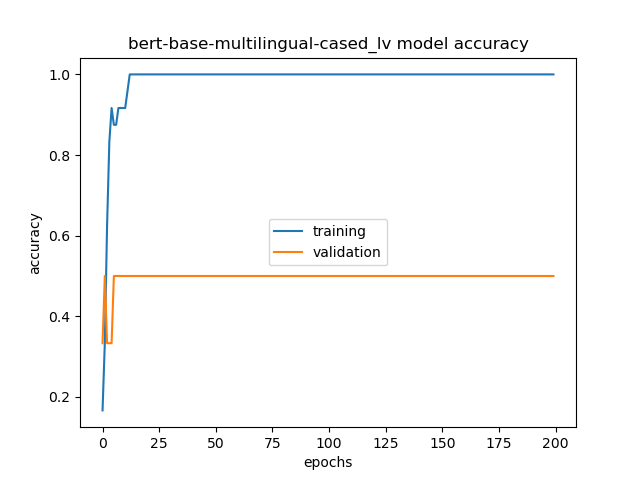
\includegraphics[width=0.49\linewidth,trim={0 0.1cm 0 0},clip]{results-5/graphs/webapps_bert-base-multilingual-cased_lv-accuracy.png}}
   \subcaptionbox{mBERT mašīntulkoto latviešu treniņdatu kopa}{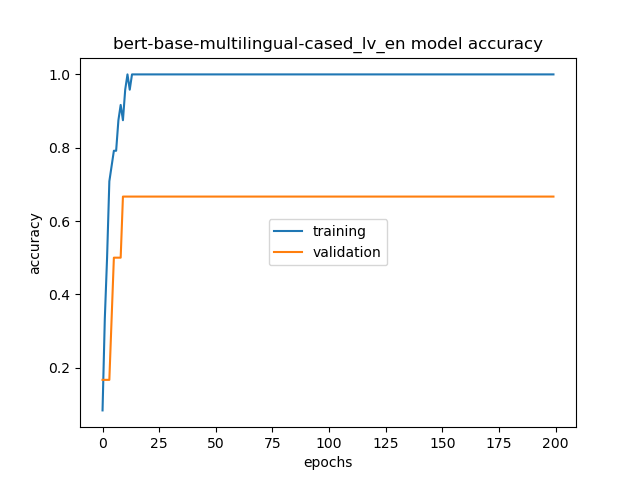
\includegraphics[width=0.49\linewidth,trim={0 0.1cm 0 0},clip]{results-5/graphs/webapps_bert-base-multilingual-cased_lv_en-accuracy.png}}
   \caption{caption} 
   \label{fig:webapps-bert}
\end{figure}


\begin{figure}[h] 
   \centering
   \subcaptionbox{mBERT apvienotā treniņdatu kopa}{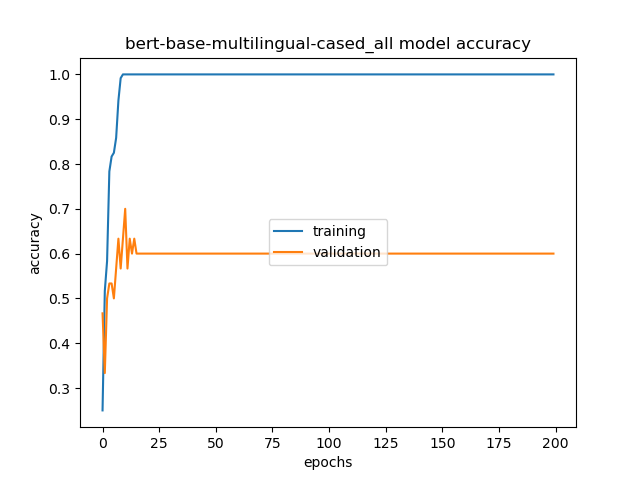
\includegraphics[width=0.49\linewidth,trim={0 0.1cm 0 0},clip]{results-5/graphs/webapps_bert-base-multilingual-cased_all-accuracy.png}}
   \subcaptionbox{mBERT apvienotā mašīntulkoto treniņdatu kopa}{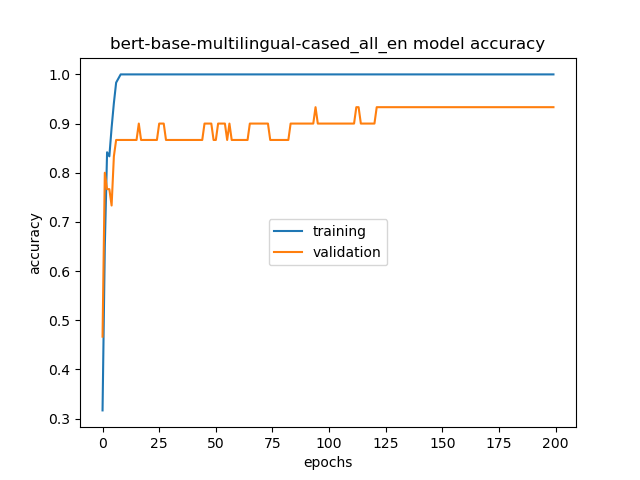
\includegraphics[width=0.49\linewidth,trim={0 0.1cm 0 0},clip]{results-5/graphs/webapps_bert-base-multilingual-cased_all_en-accuracy.png}}
   \caption{caption} 
   \label{fig:webapps-bert-all}
\end{figure}


\begin{figure}[h] 
   \centering
   \subcaptionbox{mBERT angļu treniņdatu kopa}{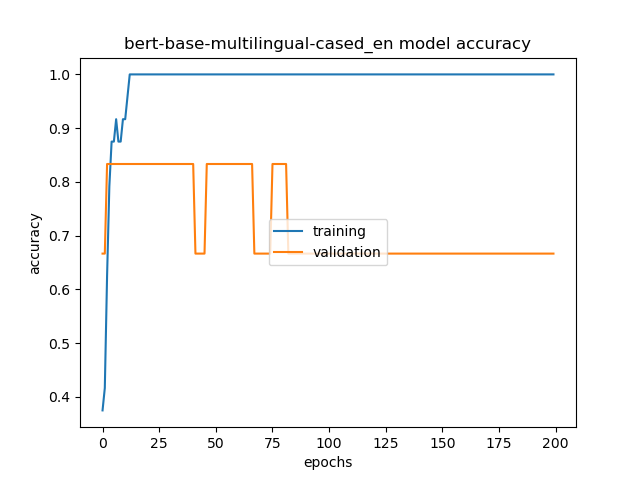
\includegraphics[width=0.49\linewidth,trim={0 0.1cm 0 0},clip]{results-5/graphs/webapps_bert-base-multilingual-cased_en-accuracy.png}}
   \subcaptionbox{XLM-RoBERTa angļu treniņdatu kopa}{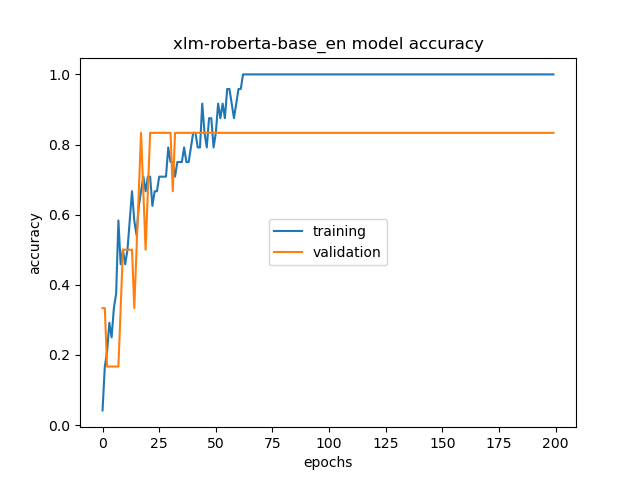
\includegraphics[width=0.49\linewidth,trim={0 0.1cm 0 0},clip]{results-5/graphs/webapps_xlm-roberta-base_en-accuracy.png}}
   \caption{caption} 
   \label{fig:webapps-bert-xlm-en}
\end{figure}


\begin{figure}[h] 
   \centering
   \subcaptionbox{XLM-RoBERTa latviešu treniņdatu kopa}{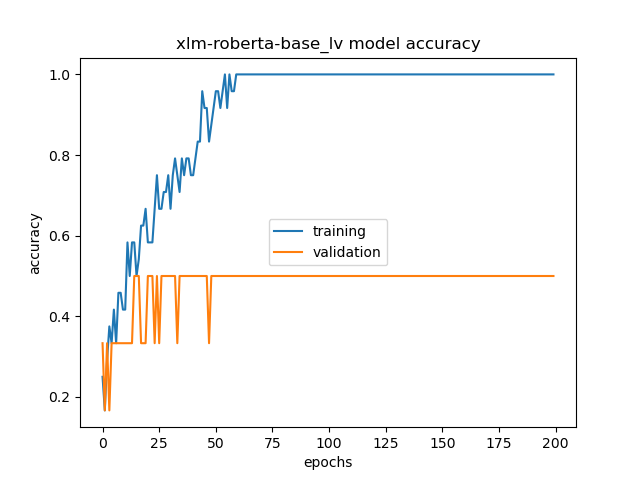
\includegraphics[width=0.49\linewidth,trim={0 0.1cm 0 0},clip]{results-5/graphs/webapps_xlm-roberta-base_lv-accuracy.png}}
   \subcaptionbox{XLM-RoBERTa mašīntulkoto latviešu treniņdatu kopa}{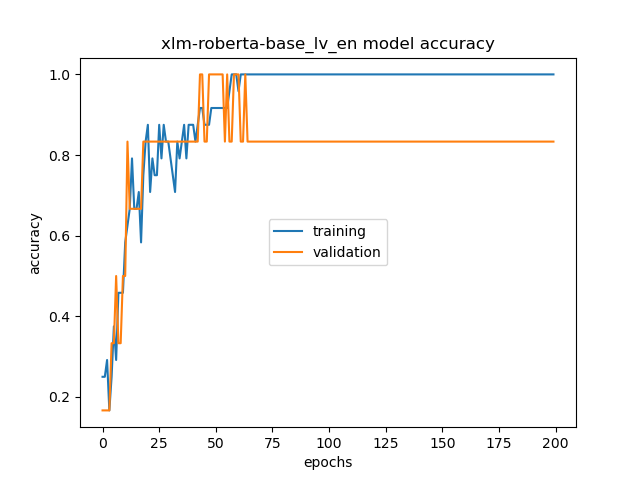
\includegraphics[width=0.49\linewidth,trim={0 0.1cm 0 0},clip]{results-5/graphs/webapps_xlm-roberta-base_lv_en-accuracy.png}}
   \caption{caption} 
   \label{fig:webapps-xlm}
\end{figure}


\begin{figure}[h] 
   \centering
   \subcaptionbox{XLM-RoBERTa apvienotā treniņdatu kopa}{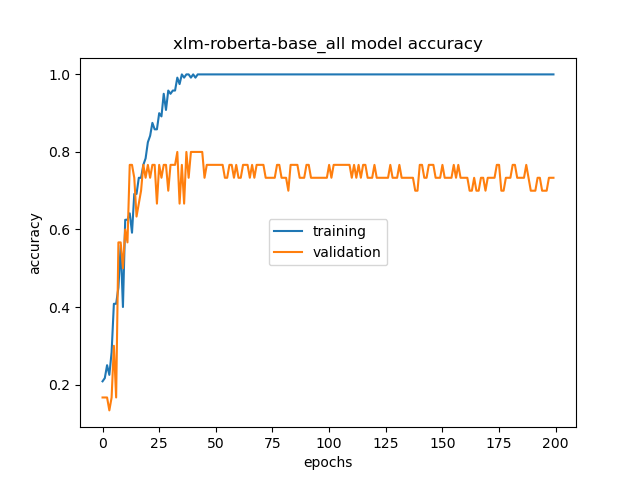
\includegraphics[width=0.49\linewidth,trim={0 0.1cm 0 0},clip]{results-5/graphs/webapps_xlm-roberta-base_all-accuracy.png}}
   \subcaptionbox{XLM-RoBERTa apvienotā mašīntulkoto treniņdatu kopa}{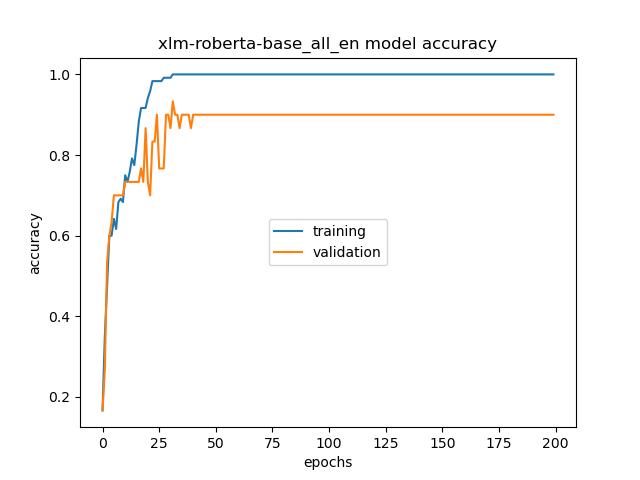
\includegraphics[width=0.49\linewidth,trim={0 0.1cm 0 0},clip]{results-5/graphs/webapps_xlm-roberta-base_all_en-accuracy.png}}
   \caption{caption} 
   \label{fig:webapps-xlm-all}
\end{figure}
